% Confirmation-window trade-off curve. Numbers are Tab. tab:nsweep (supplementary).
% Requires pgfplots (loaded in main.tex).
\begin{figure}[t]
\centering
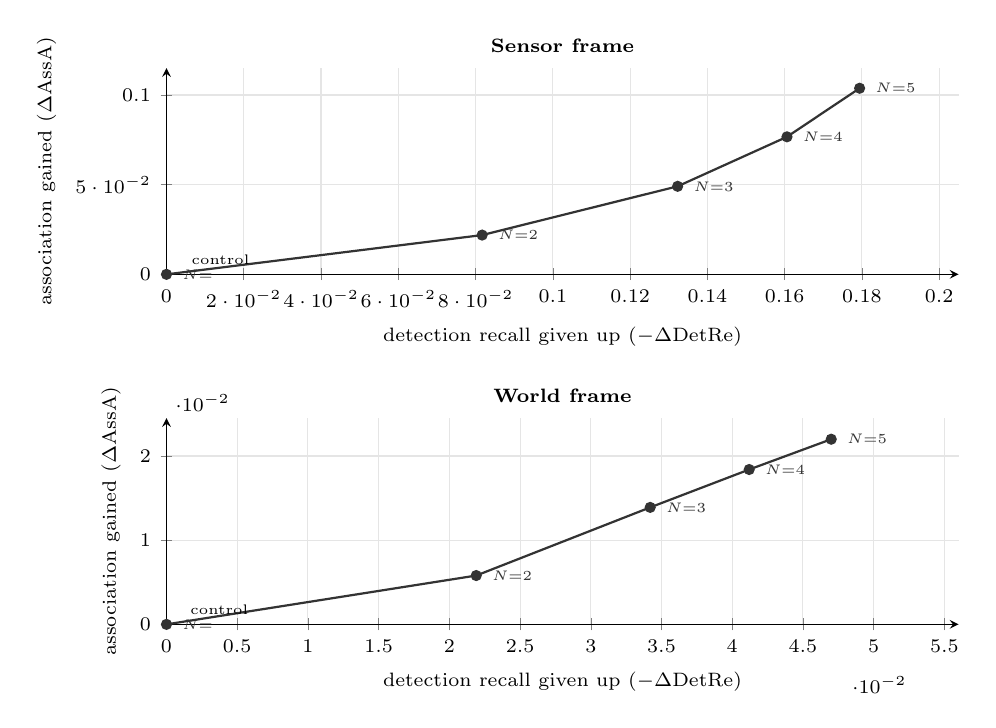
\begin{tikzpicture}
\pgfplotsset{
  every axis/.append style={
    width=0.96\linewidth, height=4.2cm,
    tick label style={font=\scriptsize}, label style={font=\scriptsize},
    title style={font=\scriptsize\bfseries, yshift=-2pt},
    axis lines=left, xmin=0, ymin=0,
    grid=major, grid style={gray!20},
  },
  every node near coord/.append style={font=\tiny, anchor=west, xshift=1pt},
}
\begin{axis}[
  name=sensor, title={Sensor frame},
  xmax=0.205, ymax=0.115,
  xlabel={detection recall given up ($-\Delta$DetRe)},
  ylabel={association gained ($\Delta$AssA)},
]
\addplot[thick, mark=*, mark size=1.6pt, color=black!80,
         nodes near coords={$N{=}\pgfplotspointmeta$}, point meta=explicit symbolic]
  coordinates {(0,0)[\!\!] (0.0817,0.0219)[2] (0.1323,0.0491)[3]
               (0.1606,0.0767)[4] (0.1794,0.1038)[5]};
\node[font=\tiny, anchor=south west] at (axis cs:0.004,0.0) {control};
\end{axis}
\begin{axis}[
  at={(sensor.below south west)}, anchor=north west, yshift=-8mm,
  title={World frame},
  xmax=0.056, ymax=0.0245,
  xlabel={detection recall given up ($-\Delta$DetRe)},
  ylabel={association gained ($\Delta$AssA)},
]
\addplot[thick, mark=*, mark size=1.6pt, color=black!80,
         nodes near coords={$N{=}\pgfplotspointmeta$}, point meta=explicit symbolic]
  coordinates {(0,0)[\!\!] (0.0219,0.0058)[2] (0.0342,0.0139)[3]
               (0.0412,0.0184)[4] (0.0470,0.0220)[5]};
\node[font=\tiny, anchor=south west] at (axis cs:0.001,0.0) {control};
\end{axis}
\end{tikzpicture}
\caption{\textbf{Confirmation is a trade-off curve, not a tuned setting.} Each
point is confirmation at that $N$ minus \emph{its own} detection-budget-matched
threshold control, so the control sits at the origin. Moving right along the
curve spends detection recall and $N{-}1$ frames of latency ($0.5$\,s each at
$2$\,Hz) and buys association accuracy; $N$ is chosen by the latency a
deployment can absorb rather than by a metric. The association gain is
positive at every $N$ in both frames and all eight bootstrap intervals exclude
zero. Full numbers, including intervals and $\Delta$AMOTA --- which, unlike
$\Delta$AssA, turns over inside the range --- are in the supplementary.}
\label{fig:nsweep}
\end{figure}
